% Provenance (never printed): see sources/outline_sources.md (Year 1: solute and particle
% fluxes; the Hjulstrom diagram; settling velocity; denudation rates). Exercise and problem
% values in the Book 3 scratch calculator calc/ch20.py; figure data from
% figdata/bachelor-1/settling.py and threshold.py. Erosion, transport and deposition are
% Book 1's (g5); the sediment load in three forms, the denudation rate and isostatic rebound
% are Book 2's (g12), re-founded here (load, denudation rate) or recalled (rebound); discharge
% and the drainage basin are Book 2 g10's; Airy isostasy is ch. 11's; viscosity, Stokes' law
% and the Reynolds number are the physics books' (admitted, pointer). Grain-size classes and
% sorting belong to ch. 21.
\chapter{侵蚀与搬运}\label{ch:b1:erosion-transport}

风暴过后，桥下的河水呈褐色。
前一天还清澈的河水，如今满是泥浆，在桥墩周围打旋，并裹挟着
树枝；河床上，看不见的卵石在滚动时彼此碰撞，
洪水每秒都带走数吨陆地物质。下游，
在一座大坝后方，同样的泥浆沉积在水库的静水中，水库
每年都会损失一小部分体积；再往下游，在河口处，
泥浆以褐色羽流的形式扩散入海，从太空亦可望见。本章
为这一历程提供数据：河流搬运多少物质、以何种形式搬运，
颗粒下沉有多快，使其开始运动需要多大的水流，以及
最终整个景观被侵蚀的速度有多快。

\begin{recall}
侵蚀是陆地被磨蚀、碎屑被搬运走的过程；
沉积则是搬运介质减速时碎屑的堆积（第 1 册，五年级）。河流
以\omterm{def:b1:erosion-transport:load}{推移质}、\omterm{def:b1:erosion-transport:load}{悬移质}和\omterm{def:b1:erosion-transport:load}{溶解质}三种形式搬运其输沙量，
一个区域的\omterm{def:b1:erosion-transport:denudation}{剥蚀速率}是单位时间内从该区域移除的岩石厚度，
以米每百万年计；当侵蚀移除厚度
为 $e$ 的\omterm{def:b1:layered-earth:layers}{地壳}时，均衡回弹使地表仅下降 
$e(1 - \rho_c/\rho_m)$（第 2 册，十二年级）。河流的流量是
单位时间内通过某一横截面的水的体积，其流域
是为其供水的区域（第 2 册，十年级）。在\omterm{prop:b1:isostasy-gravity:airy}{艾里均衡}中，\omterm{def:b1:layered-earth:layers}{地壳}
漂浮于\omterm{def:b1:layered-earth:layers}{地幔}之上，其根部与地形起伏成正比
（见\cref{prop:b1:isostasy-gravity:airy}）。硅酸盐的\omterm{def:b1:weathering-clays:hydrolysis}{水解}将离子
和溶解的二氧化硅输送到河流中（见\cref{def:b1:weathering-clays:hydrolysis}）。
流体的动力黏度 $\mu$ 表示其抵抗剪切的能力，
运动黏度则为 $\nu = \mu/\rho$；直径为 $d$ 的球体
缓慢以速度 $w$ 穿过流体运动时，受到的阻力为 $3\pi\mu d w$
（斯托克斯定律）；雷诺数 $w d/\nu$ 比较惯性力与黏性力
的相对大小，球体足够小时，其周围的流动是光滑的（参见
物理学教材）。
\end{recall}

\section{溶质与粒子通量}\label{sec:b1:erosion-transport:fluxes}

河流以两种方式搬走陆地：一种是溶解于水中的物质，它们是
\omterm{def:b1:weathering-clays:weathering}{化学风化}的产物；另一种是固体颗粒，它们是\omterm{def:b1:weathering-clays:weathering}{物理风化}的产物
以及\omterm{def:b1:weathering-clays:weathering}{化学风化}的不溶残余物。两者的搬运方式不同，
颗粒本身也有两种搬运方式。

\begin{definition}[溶解质、悬移质与推移质]\label{def:b1:erosion-transport:load}
河流的负荷是其流经某一横截面时所搬运的物质，分为三部分，
三者的区别在于搬运方式。\emph{溶解质}\index{溶解质}
是溶于水中的物质，即离子与溶解的二氧化硅，它们随水一同运动。
\emph{悬移质}\index{悬移质}由颗粒组成，这些颗粒被水流的湍流托举在水中，
主要是黏土、粉砂
和细砂，它们几乎以接近水流的速度运动，很少接触河床。
\emph{推移质}\index{推移质}由沿河床滚动、滑动或跳跃的颗粒组成，
它们频繁与河床接触，
运动速度远慢于水流。
\end{definition}

\begin{omfigure}
\begin{tikzpicture}[font=\footnotesize, >={Stealth[length=4pt]}]
% schematic: the three loads of a river (side view) and the forces on a bed grain
\fill[omDef!12] (0,0) rectangle (9,3.2);
\draw[omDef!80!black, thick] (0,3.2) -- (9,3.2);
\node[anchor=south west, omDef!80!black] at (0,3.2) {水面};
% flow profile arrows (velocity grows upward)
\foreach \y/\l in {0.35/0.5, 0.8/0.9, 1.4/1.15, 2.1/1.3, 2.8/1.4} {\draw[->, black!55] (0.25,\y) -- ++(\l,0);}
\draw[black!55] (0.25,0.12) -- (0.25,3.05);
\node[anchor=north west, black!65, align=left] at (0.2,-0.15) {流速 \\ 剖面};
% bed
\fill[black!12] (0,-0.05) rectangle (9,0.12);
\foreach \x in {0.1,0.45,...,8.9} {\fill[black!45] (\x,0.0) circle[radius=0.09];}
% dissolved load: ions
\foreach \x/\y/\s in {2.3/2.7/+, 3.1/1.9/-, 4.0/2.85/+, 4.7/2.2/-, 5.6/2.75/+, 6.3/1.85/+, 7.2/2.6/-, 8.2/2.2/+, 2.7/1.2/-, 7.8/1.3/-} {\node[circle, draw=omThm, inner sep=0.2pt, minimum size=7pt, font=\tiny, text=omThm] at (\x,\y) {$\s$};}
% suspended load: fine grains, denser near the bed
\foreach \x/\y in {2.1/1.5, 2.6/0.9, 3.0/2.5, 3.4/0.6, 3.7/1.4, 4.2/0.8, 4.4/1.9, 4.9/0.55, 5.2/1.2, 5.5/2.1, 5.9/0.7, 6.1/1.5, 6.6/0.9, 6.9/2.3, 7.4/0.6, 7.6/1.7, 8.0/0.85, 8.5/1.4, 3.9/0.45, 5.0/0.35, 6.4/0.4, 2.4/0.45, 8.6/0.5} {\fill[brown!75!black] (\x,\y) circle[radius=0.05];}
% bed load: rolling and hopping grains
\fill[black!60] (3.2,0.27) circle[radius=0.15];
\draw[->, black!70] (3.0,0.55) arc[start angle=150, end angle=30, radius=0.25];
\fill[black!60] (5.6,0.25) circle[radius=0.12];
\draw[->, black!70, densely dashed] (4.6,0.2) .. controls (4.9,0.9) and (5.3,0.7) .. (5.55,0.4);
\fill[black!60] (4.6,0.22) circle[radius=0.06];
% labels
\node[omThm, anchor=west] at (9.2,2.5) {溶解质：离子};
\node[brown!75!black, anchor=west] at (9.2,1.5) {悬移质：};
\node[brown!75!black, anchor=west] at (9.2,1.1) {黏土、粉砂、细砂};
\node[black!75, anchor=west] at (9.2,0.4) {推移质：滚动，};
\node[black!75, anchor=west] at (9.2,0.0) {滑动、跳跃的颗粒};
\draw[->, thick, black!70] (6.8,3.55) -- node[above] {水流} (8.6,3.55);
% inset: forces on a grain resting on two others; it pivots about its downstream contact
\begin{scope}[xshift=11.8cm, yshift=-2.2cm]
  \fill[black!12] (-1.2,-0.4) rectangle (1.2,0);
  \fill[black!40] (-0.6,-0.15) circle[radius=0.28]; \fill[black!40] (0.6,-0.15) circle[radius=0.28];
  \fill[black!65] (0,0.166) circle[radius=0.4];
  \draw[->, thick, omDef!80!black] (0,0.166) -- (0,1.15) node[above] {升力};
  \draw[->, thick, omThm] (0,0.166) -- (1.05,0.166) node[right] {阻力};
  \draw[->, thick, black] (0,0.166) -- (0,-0.8) node[below] {浸没重量};
  \draw[->, thick, black!60] (-1.4,0.85) -- (-0.5,0.85) node[pos=0, left] {水流};
  \fill[red!60!black] (0.353,-0.020) circle[radius=0.045];
  \node[font=\scriptsize, anchor=north west, black!70] at (0.5,-0.4) {支点};
\end{scope}
\end{tikzpicture}

{\small 河流的三种负荷，侧视示意（非按比例绘制）。
水流在水面附近最快，到河床处减为零。离子
遍布整个水深；\omterm{def:b1:erosion-transport:load}{悬移质}颗粒被涡流携带，
其中靠近河床的较多；\omterm{def:b1:erosion-transport:load}{推移质}颗粒滚动、滑动或短距离跳跃。
右图：河床上一粒颗粒所受的力。水流的阻力与升力\omterm{def:b1:geological-maps:attitude}{倾向}于使其
绕接触点越过下游的邻粒翻滚；
其在水中的重量则将其压住。}
\label{fig:b1:erosion-transport:loads}
\end{omfigure}

两种固体负荷之间的界限并不由颗粒粒径决定：它
取决于水流。挟砂悬浮的洪水在退落时，把砂留在
河床上，成为\omterm{def:b1:erosion-transport:load}{推移质}；而最细的黏土则
几乎在任何水流中都保持悬浮状态，很少见于流动河流的河床上。
每种负荷都以通量来度量，即单位时间内穿过
河流某一剖面的质量。

\begin{proposition}[负荷的通量]\label{prop:b1:erosion-transport:flux}
设 $c$ 为\omterm{def:b1:erosion-transport:load}{溶解质}或\omterm{def:b1:erosion-transport:load}{悬移质}的浓度（单位
水体体积内的质量），$u$ 为水流速度，二者均
随面积为 $A$ 的截面位置而变化。（1）瞬时通过该截面的
负荷通量为
\[
  F = \iint_A c\,u\,\mathrm dA = \overline{c}_Q\,Q,
\]
其中 $Q = \iint_A u\,\mathrm dA$ 为流量，$\overline{c}_Q$
为以速度加权的平均浓度。（2）在时段 $T$ 内，
河流的流量 $Q(t)$ 与浓度 $C(t)$ 发生变化，所携带的
质量为
\[
  M = \int_0^T Q\,C\,\mathrm dt = T\left(\overline{Q}\;\overline{C} +
  \operatorname{cov}(Q, C)\right),
\]
其中上横线表示对时间的平均，$\operatorname{cov}(Q, C)$ 为
$(Q - \overline{Q})(C - \overline{C})$ 的平均值。平均流量与
平均浓度之积，只有在二者
互不相关时，才能给出正确的质量。
\end{proposition}

\begin{proof}
（1）在时间 $\mathrm dt$ 内，穿过截面上微小面积 $\mathrm dA$ 的
水，充满的体积为 $u\,\mathrm dA\,\mathrm dt$，其携带的
质量为 $c\,u\,\mathrm dA\,\mathrm dt$；对截面求和得到 $F$，并
$\overline{c}_Q$ 定义为 $F/Q$。（2）记 $Q = \overline{Q} + Q'$，$C =
\overline{C} + C'$，其中涨落量 $Q'$ 与 $C'$ 在
时段内的平均值为零。于是有 $QC = \overline{Q}\,\overline{C} + \overline{Q}\,C' + Q'\,\overline{C}
+ Q'C'$；中间两项平均后为零，$Q'C'$ 的平均值即
协方差。
\end{proof}

协方差对\omterm{def:b1:erosion-transport:load}{悬移质}负荷很重要。其浓度在洪水期间急剧
上升：降雨把土壤冲入溪流，流速加快的水流把颗粒从
河床上托起，因此 $Q$ 与 $C$ 同时增大：河流每年的大部分沉积物
往往在几天洪水中输移，而错过这些时段的采样
工作，或以平均浓度乘以平均流量的做法，
都会低估负荷。\omterm{def:b1:erosion-transport:load}{溶解质}则恰恰相反：洪水会稀释它，
其浓度在枯水期最高，此时河流由
与岩石长期接触的地下水补给。

\begin{method}[根据测站观测估算河流年负荷]\label{met:b1:erosion-transport:gauging}
\begin{enumerate}
  \item 在测站连续记录流量。
  \item 在多种流量下采集水样（包括洪水期），测定
        每升水中沉积物的质量（过滤后称重）及
        各溶解物质种类的质量。
  \item 以采样时的流量对浓度加权，
        得到以流量加权的平均浓度；或将浓度
        拟合为流量的函数，并将其用于全部记录。
  \item 乘以全年的总水量，或对记录求和 $Q\,C\,\Delta
        t$（见\cref{prop:b1:erosion-transport:flux}）。
  \item 加上\omterm{def:b1:erosion-transport:load}{推移质}，这部分水样采集器通常漏测，可由
        单独测量得到，或按估计比例计入。
  \item 对\omterm{def:b1:erosion-transport:load}{溶解质}，需扣除并非来自岩石的部分：
        雨水带来的盐分，以及对碳酸氢根而言，取自
        空气的碳（见\cref{ch:b1:weathering-clays}）。
\end{enumerate}
\end{method}

\begin{omfigure}
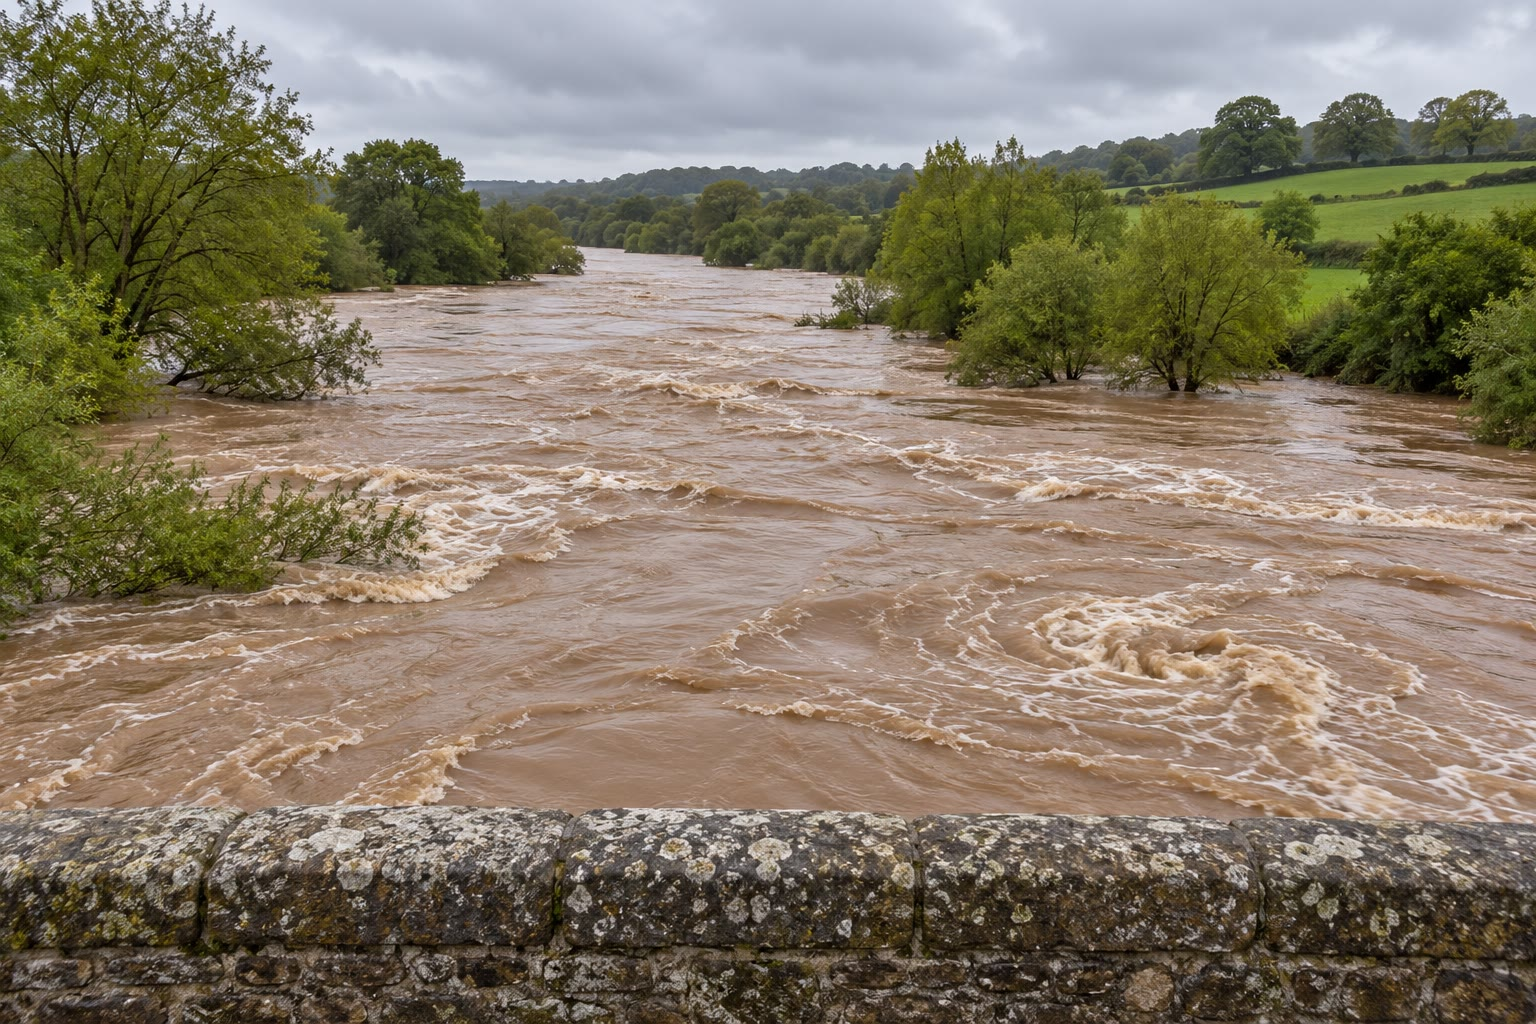
\includegraphics[height=5.1cm]{images/book3/ai/b1-muddy-river.jpg}\hfill
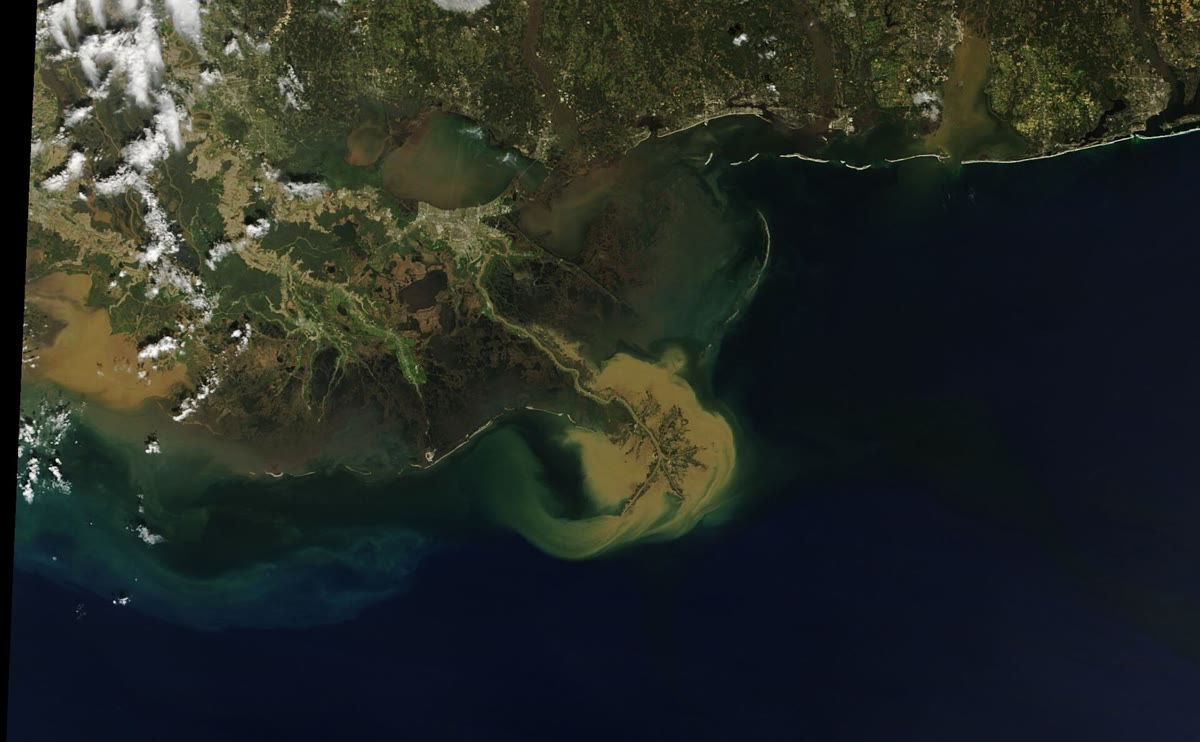
\includegraphics[height=5.1cm]{images/book3/b1-mississippi-plume.jpg}
\par\smallskip{\small 左：洪水中的河流携带着棕色、富含沉积物的
水流（AI 插图）。右：密西西比河的洪水羽流
注入墨西哥湾，环绕其三角洲，由
Terra 卫星上的 MODIS 仪器于 2018 年 3 月 4 日所摄；悬浮泥沙使海水呈棕色和
绿色，东南风将羽流推向西北。NASA 地球观测站图像，作者
Joshua Stevens，公有领域，经维基共享资源提供。}
\label{fig:b1:erosion-transport:plume}
\end{omfigure}
% ledger: commons:mississippi-plume

\emph{世界河流。}未受人类影响时，世界河流
估计每年向沿海海洋输送约 \qty{14}{Gt} 的悬浮沉积物，
海洋，连同\omterm{def:b1:erosion-transport:load}{推移质}则为 \qty{15.5}{Gt}。人类已改变了
输送过程的两端：农业与森林砍伐加剧了土壤侵蚀，每年向河流增加约
\qty{2.3}{Gt}，而水库则拦截沉积物：大型水库拦截约
\qty{20}{\percent} 的通量，小型水库另拦截
\qty{6}{\percent}；目前已有超过 \qty{100}{Gt} 的沉积物淤积在
大多建于近五十年的水坝之后。净效应是通量减少：
现今通量约为每年 \qty{12.6}{Gt}。
% ledger: syvitski:flux

\begin{dated}{2005}
关于悬浮沉积物通量在人类影响前后的数值，
取自 2005 年发表的河流沉积物全球模型。此后已
修建了不少水坝。
\end{dated}
% ledger: syvitski:flux

\omterm{def:b1:erosion-transport:load}{溶解质}负荷较小。一部经典的河流分析汇编，编成于
1963 年，将世界河流输入海洋的溶解物质
约为每年 \qty{3.9}{Gt}，相当于现今
悬浮通量的约 \qty{30}{\percent}，平均浓度为每升 \qty{120}{mg}。碳酸氢根
约占其近半，为 \qty{58}{mg.L^{-1}}，其后依次为钙、二氧化硅、硫酸根、
氯离子和钠离子。其中一部分并非来自岩石：大部分
碳酸氢根所携带的碳取自空气或土壤，而部分
氯离子和钠离子则来自雨水携带的海盐。各河流
的数值围绕这些均值差异很大。
% ledger: livingstone:world-dissolved, syvitski:flux

\emph{盆地的泥沙收支。}并非流域内被侵蚀的每一颗颗粒
都能到达出口。从农田冲刷下来的土壤
可能停在坡脚，沙可能在河漫滩和河道沙坝中储存数百年，
水库可能截留进入其中的大部分泥沙。出口处测得的负荷
是收支的结果：坡面和河岸上被侵蚀的量，
减去途中被储存的量，再加上从旧有储存中重新带出的量。
若只观测几十年，这一收支可能
与长期侵蚀速率相差甚远，且偏差可朝任一方向，
这也是需要借助\cref{sec:b1:erosion-transport:denudation}中其他方法的原因之一。

\section{沉降速度}\label{sec:b1:erosion-transport:settling}

颗粒的密度大于水，因而会下沉。河流能否搬运它，以及
它将在何处沉积，首先取决于它下沉的快慢。

\begin{definition}[沉降速度]\label{def:b1:erosion-transport:settling}
颗粒的\emph{沉降速度}\index{沉降速度} $w_s$，是指颗粒在静水中
匀速下落时的速度，此时水对它的阻力
与其浸没重量平衡，浸没重量即其自身重量
减去所排开水的浮力。
\end{definition}

颗粒在静水中释放后加速，直至随速度增大的阻力
与其浸没重量平衡；对于沙或粉砂颗粒，这一过程
只需极短的时间，因此\omterm{def:b1:erosion-transport:settling}{沉降速度}即颗粒
几乎全程下落时的速度。设颗粒密度为 $\rho_s$，
水的密度为 $\rho$，记 $R = (\rho_s - \rho)/\rho$ 为相对
浸没密度。

\begin{proposition}[斯托克斯沉降]\label{prop:b1:erosion-transport:stokes}
直径为 $d$、密度为 $\rho_s$ 的球体在密度为 $\rho$ 的水中
缓慢下落，水的动力黏度为 $\mu$，按斯托克斯定律，其\omterm{def:b1:erosion-transport:settling}{沉降
速度}为
\[
  w_s = \frac{(\rho_s - \rho)\,g\,d^2}{18\,\mu} = \frac{R\,g\,d^2}{18\,\nu}.
\]
当颗粒雷诺数 $w_s d/\nu$ 小于约 1 时，该定律成立，
即直径小于 $d_1 = \left(18\,\nu^2/(R\,g)\right)^{1/3}$ 时成立。
\end{proposition}

\begin{proof}
球体的重量为 $\rho_s g\,\pi d^3/6$，浮力为
$\rho g\,\pi d^3/6$，故其浸没重量为 $(\rho_s - \rho)\,g\,\pi d^3/6$。
在\omterm{def:b1:erosion-transport:settling}{沉降速度}下，它与阻力 $3\pi\mu d\,w_s$ 相等：
\[
  (\rho_s - \rho)\,g\,\frac{\pi d^3}{6} = 3\pi\mu d\,w_s
  \quad\Longrightarrow\quad
  w_s = \frac{(\rho_s - \rho)\,g\,d^2}{18\,\mu},
\]
分子分母同除以 $\rho$，即得第二种形式。
该速度下的雷诺数为 $R g d^3/(18\nu^2)$，当
$d = d_1$ 时它等于 1，并随 $d^3$ 增大。
\end{proof}

对于密度为 \qty{2650}{kg.m^{-3}} 的石英，在 \qty{20}{\celsius}
的水中（密度为 \qty{998.2}{kg.m^{-3}}，黏度为 \qty{1.0016}{mPa.s}）：$R =
1.65$，$\nu = \qty{1.003e-6}{m^2.s^{-1}}$，取 $g =
\qty{9.81}{m.s^{-2}}$，则界限为 $d_1 = \qty{0.104}{mm}$，属细沙。
在此以下，斯托克斯定律给出粉砂和黏土的\omterm{def:b1:erosion-transport:settling}{沉降速度}：粉砂颗粒
直径 \qty{10}{\micro m}，以 \qty{9.0e-5}{m.s^{-1}} 下沉，下落 \qty{1}{m}
约需三小时；直径 \qty{2}{\micro m} 的黏土颗粒以
\qty{3.6e-6}{m.s^{-1}} 下沉，下落 \qty{1}{m} 需 \num{3.2}~天。天然黏土颗粒
呈\omterm{def:b1:field-lab-methods-1:thin-section}{薄片}状而非球形，下沉更慢。水深 \qty{5}{m}、完全
静止的水需十六天才能澄清此类黏土；而流动的河水，
其涡流不断搅动它，因此永远不会澄清，这正是最细的泥浆
能被带到海里的原因。
% ledger: hom:quartz, nist:water, const:gn

粒径大于 $d_1$ 时，阻力增长快于与速度成正比的关系：流经颗粒的水
在其后方分离形成尾流，雷诺数较大时，
阻力与速度的平方成正比。对天然颗粒的实验结果
可归纳为一个同时涵盖两种情形的公式。

\begin{proposition}[综合沉降定律]\label{prop:b1:erosion-transport:combined}
筛分直径为 $d$ 的天然颗粒，其\omterm{def:b1:erosion-transport:settling}{沉降速度}对所有
粒径均为
\[
  w_s = \frac{R\,g\,d^2}{C_1\,\nu + \sqrt{0.75\,C_2\,R\,g\,d^3}},
\]
其中 $C_1 = 18$，$C_2 = 1.0$。
\end{proposition}
\admitted
% ledger: fc:settling

该定律由弗格森和彻奇提出，他们用它拟合了实测的
天然沙的\omterm{def:b1:erosion-transport:settling}{沉降速度}。对小颗粒，平方根项
可忽略，公式退化为斯托克斯定律；对大颗粒，分母中的第一项
可忽略，此时 $w_s \to \sqrt{4 R g d/(3 C_2)}$，
仅随粒径的平方根增长。常数取决于
颗粒形状：$C_2 = 0.4$ 对应光滑的球形颗粒，取值越大，颗粒越
有棱角，所受阻力越大。两种定律在
\qty{0.1}{mm} 以上开始明显偏离。对于 \qty{1}{mm} 的颗粒，综合沉降定律给出
\qty{0.126}{m.s^{-1}}，比斯托克斯定律小七倍；对于
\qty{10}{mm} 的卵石，综合沉降定律给出 \qty{0.46}{m.s^{-1}}，
而斯托克斯定律给出的 \qty{90}{m.s^{-1}} 毫无意义（见下图）。
% ledger: fc:settling

\begin{omfigure}
\begin{tikzpicture}[font=\small]
% settling velocity of quartz grains in water at 20 C (figdata/bachelor-1/settling.py)
\begin{axis}[width=11cm, xmode=log, ymode=log, xmin=0.001, xmax=10, ymin=1e-8, ymax=10, height=8cm,
    xlabel={颗粒直径 $d$ (\si{mm})}, ylabel={沉降速度 (\si{m.s^{-1}})},
    ytick={1e-8,1e-6,1e-4,1e-2,1},
    legend style={at={(0.03,0.97)}, anchor=north west, font=\footnotesize}, legend cell align=left,
    grid=major, grid style={black!10}]
  \addplot[omDef, thick, dashed] table[x=d_mm, y=w_stokes] {figdata/out/bachelor-1-settling-curves.dat};
  \addplot[omThm, very thick] table[x=d_mm, y=w_fc] {figdata/out/bachelor-1-settling-curves.dat};
  \legend{斯托克斯定律, 综合沉降定律（天然颗粒）}
  \draw[black!55, densely dotted] (axis cs:0.1037,1e-7) -- (axis cs:0.1037,10);
  \node[font=\scriptsize, anchor=west, align=left, black!75] at (axis cs:0.115,1e-6) {颗粒雷诺数 \\ $= 1$};
  \node[font=\scriptsize, black!70] at (axis cs:0.002,3e-8) {黏土};
  \node[font=\scriptsize, black!70] at (axis cs:0.016,3e-8) {粉砂};
  \node[font=\scriptsize, black!70] at (axis cs:0.35,3e-8) {沙};
  \node[font=\scriptsize, black!70] at (axis cs:4.5,3e-8) {砾石};
  \draw[black!40] (axis cs:0.0039,1e-8) -- (axis cs:0.0039,1e-7);
  \draw[black!40] (axis cs:0.0625,1e-8) -- (axis cs:0.0625,1e-7);
  \draw[black!40] (axis cs:2,1e-8) -- (axis cs:2,1e-7);
\end{axis}
\end{tikzpicture}

{\small 水中石英颗粒在 \qty{20}{\celsius} 下的\omterm{def:b1:erosion-transport:settling}{沉降速度}，
随其直径的变化关系，两坐标轴均为对数刻度：斯托克斯定律与
天然颗粒综合定律的计算结果。在这些刻度下，斯托克斯定律是一条
斜率为 2 的直线。二者在粉砂与黏土范围内吻合；在约
\qty{0.1}{mm} 以上，颗粒雷诺数超过 1，尾流阻力
使粗颗粒减速。图底部的刻度标出了粒级界线，
分别位于 \qty{3.9}{\micro m}（$1/256$~mm）、\qty{62.5}{\micro m}
（$1/16$~mm）和 \qty{2}{mm} 处。}
\label{fig:b1:erosion-transport:settling}
\end{omfigure}
% ledger: fc:settling, usgs:wentworth-phi

图中所示范围内，从最细的黏土到粗砾石，
\omterm{def:b1:erosion-transport:settling}{沉降速度}跨越八个数量级。这是河流分选沉积物的第一个原因：
减速的水流会立即沉积其中的砾石，
沙在数米之内沉降，粉砂在数千米之内沉降，并将黏土携带到
湖泊或海中。粒级划分与沉积物分选
是下一章（\cref{ch:b1:clastic-sediments}）的主题。

\section{起动阈值与尤尔斯特伦图}\label{sec:b1:erosion-transport:threshold}

河床上静止的颗粒被流过其上的水流的力推动而
开始运动，这一作用力用一个应力来度量。

\begin{definition}[床面剪应力，摩阻流速]\label{def:b1:erosion-transport:bed-shear}
称流动的\emph{床面剪应力}\index{床面剪应力} $\tau_b$ 为
单位面积上水流施加于床面的力，与床面平行，
沿流动方向。摩阻流速为 $u_* = \sqrt{\tau_b/\rho}$，
它是度量同一应力的一种速度。
\end{definition}

\omterm{def:b1:erosion-transport:bed-shear}{床面剪应力}不能直接由流速计读出，但在稳定流动中
可由力的平衡关系求得。

\begin{proposition}[水深–坡度乘积]\label{prop:b1:erosion-transport:depth-slope}
在水深为 $h$ 的稳定均匀流中，河道宽阔，坡度 $S$ 很小，
\omterm{def:b1:erosion-transport:bed-shear}{床面剪应力}为
\[
  \tau_b = \rho\,g\,h\,S .
\]
\end{proposition}

\begin{proof}
考察一段沿流向长为 $L$、单位宽度的床面上方的水体，
河道足够宽，可忽略其河岸的作用。水流
稳定且均匀，故该水体不加速，其受力
保持平衡。上下游两个侧面所受压力大小相等、
方向相反，因两侧水深相同。沿流向剩下的力有
重力沿流向的分量 $\rho g h L \sin\beta$，其中 $\beta$ 为床面\omterm{def:b1:geological-maps:attitude}{倾角}，
以及床面的摩擦力 $\tau_b L$，与之反向。由此得 $\tau_b
= \rho g h \sin\beta$，对小角度有 $\sin\beta \approx \tan\beta = S$。
\end{proof}

水深 \qty{2}{m}、坡度为 \num{0.001}（每千米落差一米）的河流，
其\omterm{def:b1:erosion-transport:bed-shear}{床面剪应力}为 $\tau_b = 998.2 \times 9.81 \times 2 \times 0.001 =
\qty{19.6}{Pa}$，摩阻流速为 \qty{0.140}{m.s^{-1}}。在河道不宽的情形下，
两岸也分担摩擦，此时水深应
以水力半径代替，即过水断面面积除以湿周
（见\cref{exo:b1:erosion-transport:5}）。

\emph{作用于颗粒的力。}水流以其阻力推动床面上的颗粒，
并借颗粒顶部较快水流将其托起（即本章第一幅图中的插图）。
两种力均作用于颗粒的受力面积上，故其量级正比于 $\tau_b
d^2$；颗粒以其浮重抵抗，浮重
与 $(\rho_s - \rho) g d^3$ 成正比。两者之比是
给定颗粒条件下水流强度的自然度量。

\begin{definition}[希尔兹参数，起动阈值]\label{def:b1:erosion-transport:threshold}
称\emph{希尔兹参数}\index{希尔兹参数}为：\omterm{def:b1:erosion-transport:bed-shear}{床面剪应力}为 $\tau_b$ 的水流
作用于直径为 $d$、密度为 $\rho_s$ 的颗粒上时，其值为
\[
  \theta = \frac{\tau_b}{(\rho_s - \rho)\,g\,d}.
\]
颗粒的\emph{起动阈值}\index{起动阈值}是
\omterm{def:b1:erosion-transport:bed-shear}{床面剪应力}，或使颗粒开始运动时希尔兹参数的值 $\theta_c$，
在此值下颗粒开始运动。
\end{definition}
% ledger: hecras:thresholds

临界值 $\theta_c$ 由水槽实验测得，测量结果
将其对无量纲粒径作图时落在同一条曲线上，该无量纲粒径
综合了颗粒与流体的性质。

\begin{proposition}[索尔斯比与怀特豪斯的阈值曲线]\label{prop:b1:erosion-transport:soulsby}
对平坦床面上直径为 $d$ 的颗粒，记
$D_* = d\,\left(R\,g/\nu^2\right)^{1/3}$，则临界\omterm{def:b1:erosion-transport:threshold}{希尔兹参数}为
\[
  \theta_c = \frac{0.3}{1 + 1.2\,D_*} + 0.055\left(1 - e^{-0.02\,D_*}\right),
\]
临界\omterm{def:b1:erosion-transport:bed-shear}{床面剪应力}为 $\tau_c = \theta_c\,(\rho_s - \rho)\,g\,d$。
\end{proposition}
\admitted
% ledger: hecras:thresholds

对粗颗粒，$\theta_c$ 趋于 \num{0.055}：砾石开始运动时，\omterm{def:b1:erosion-transport:bed-shear}{床面
剪应力}达到约一个颗粒直径厚的颗粒层浮重的
二十分之一（按单位面积计）。采用常值阈值的输沙公式取值从
\num{0.03} 至 \num{0.047}，后者见
经典的迈耶-彼得与米勒\omterm{def:b1:erosion-transport:load}{推移质}公式。对细砂，$\theta_c$ 再次升高至
\num{0.077}（对应 \qty{0.1}{mm}）：细小颗粒位于贴近床面的缓慢黏性水层之中，
并受到相邻颗粒的遮蔽。最小值
\num{0.030}，出现在 \qty{0.7}{mm} 附近。以帕斯卡计，阈值总是
随粒径增大（见下图）：粒径为 \qty{0.1}{mm} 的沙为 \qty{0.13}{Pa}，
粒径 \qty{1}{mm} 时为 \qty{0.51}{Pa}，\qty{10}{mm} 时为 \qty{9.0}{Pa}，
\qty{64}{mm} 的卵石则为 \qty{57}{Pa}。
% ledger: hecras:thresholds

\begin{omfigure}
\begin{tikzpicture}[font=\small]
% threshold of motion of quartz grains in water at 20 C (figdata/bachelor-1/threshold.py, Soulsby and Whitehouse)
\begin{axis}[name=a, width=6.9cm, height=6cm, xmode=log, xmin=0.0625, xmax=100, ymin=0, ymax=0.12,
    xlabel={粒径 $d$ (\si{mm})}, ylabel={临界希尔兹参数 $\theta_c$},
    yticklabel style={/pgf/number format/fixed, /pgf/number format/precision=2},
    grid=major, grid style={black!10}, title={\footnotesize (a) 无量纲}]
  \addplot[omThm, very thick] table[x=d_mm, y=theta] {figdata/out/bachelor-1-threshold-shields.dat};
  \draw[black!50, dashed] (axis cs:0.0625,0.055) -- (axis cs:100,0.055) node[pos=0.7, above, font=\scriptsize, black!70] {$0.055$};
\end{axis}
\begin{axis}[at={(a.east)}, anchor=west, xshift=2.0cm, width=6.9cm, height=6cm, xmode=log, ymode=log,
    xmin=0.0625, xmax=100, ymin=0.05, ymax=200,
    xlabel={粒径 $d$ (\si{mm})}, ylabel={临界床面剪应力 $\tau_c$ (\si{Pa})},
    grid=major, grid style={black!10}, title={\footnotesize (b) 以帕斯卡计}]
  \addplot[omDef, very thick] table[x=d_mm, y=tau_cr] {figdata/out/bachelor-1-threshold-shields.dat};
\end{axis}
\end{tikzpicture}

{\small 石英颗粒在水中的\omterm{def:b1:erosion-transport:threshold}{起动阈值}，
水温 \qty{20}{\celsius}，取自索尔斯比与怀特豪斯的曲线，计算范围从细砂边界
（\qty{0.0625}{mm}）到卵石粒径。（a）~临界\omterm{def:b1:erosion-transport:threshold}{希尔兹参数}
对砾石近似恒定，对细砂则上升。（b）~临界\omterm{def:b1:erosion-transport:bed-shear}{床面剪应力}
对砾石几乎与粒径成正比增长。}
\label{fig:b1:erosion-transport:threshold}
\end{omfigure}
% ledger: hecras:thresholds

\begin{example}[河流搬运的物质]\label{ex:b1:erosion-transport:river}
在水深 \qty{2}{m}、坡度为 \num{0.001} 的河流中，$\tau_b =
\qty{19.6}{Pa}$。对于粒径为 \qty{20}{mm} 的颗粒，$\theta = 19.6/(1651.8 \times
9.81 \times 0.020) = 0.060$，略高于其\omterm{def:b1:erosion-transport:threshold}{起动阈值} \num{0.055}：它们
开始运动。对于粒径为 \qty{40}{mm} 的颗粒，$\theta = 0.030$，为阈值的一半，它们
保持静止。河流能搬动的河床物质可粗至砾石；对于 \qty{1}{mm} 的砂，
$\theta = 1.21$，约为其阈值 \num{0.031} 的近四十倍。
\end{example}

\emph{进入悬浮。}颗粒一经起动，便沿床面跳跃，或被卷入水流，
取决于旋涡能否托住颗粒、抵消其沉降，这些旋涡
的速度与剪切速度同量级。

\begin{proposition}[悬浮判据]\label{prop:b1:erosion-transport:suspension}
\omterm{def:b1:erosion-transport:settling}{沉降速度}为 $w_s$ 的颗粒，在湍流中
只有某些旋涡上升速度快于其下沉，才能悬浮。旋涡的
向上速度与剪切速度 $u_*$ 同量级，悬浮
于 $u_*$ 接近 $w_s$ 时开始，$u_*$ 超过它时充分发展；
本章取 $u_* = w_s$ 作为悬浮的极限。
\end{proposition}
\admitted
% ledger: bagnold:suspension

在例中的河流里，$u_* = \qty{0.140}{m.s^{-1}}$，综合沉降律给出的
颗粒粒径为 \qty{1.16}{mm}：比约一毫米更细的砂以悬浮方式输运，
较粗的砂与砾石则以\omterm{def:b1:erosion-transport:load}{推移质}方式输运。
这一论证可追溯至巴格诺尔德，他指出 \qty{0.1}{mm} 或
更细的颗粒一经起动即完全悬浮，而大于
\qty{1}{mm} 的颗粒则需要比其\omterm{def:b1:erosion-transport:threshold}{起动阈值}大许多倍的\omterm{def:b1:erosion-transport:bed-shear}{床面剪应力}。当
洪水退去、$u_*$ 下降时，粗砂率先落回床面。

\emph{从应力到平均流速。}河流中易于测量或估算的，
是其平均流速。在由颗粒构成粗糙床面的湍流中，
粒径为 $d$ 的颗粒，深度为 $h$ 的宽河道，其平均流速为
$U = u_*\left(6.25 + 5.75\log_{10}(h/d)\right)$，此律由凯勒根
于 1938 年依据尼古拉兹与巴赞的实验建立，因此\omterm{def:b1:erosion-transport:threshold}{起动阈值}对应于
临界平均流速
\[
  U_c = \left(6.25 + 5.75\,\log_{10}\frac{h}{d}\right)\sqrt{\theta_c\,R\,g\,d},
\]
而悬浮极限 $u_* = w_s$，对应的 $U_s = \left(6.25 +
5.75\log_{10}(h/d)\right) w_s$。两者都依赖水深，但仅经由
一个对数项体现。
% ledger: keulegan:mean-velocity, bagnold:suspension

因此，起动速度只属于某一水深及同一套规律：
若按另一水深计算，或取自其他测量，结果会
有所不同。若以粒径为横坐标作图，其形状稳健，但
数值并不稳健。\omterm{def:b1:erosion-transport:bed-shear}{床面剪应力}对水深的依赖方式不同，
因而是衡量水流能力更好的指标。流速
仍更直观，其经典表示方法是一张图。

\begin{definition}[尤尔斯特伦图]\label{def:b1:erosion-transport:hjulstrom}
\emph{尤尔斯特伦图}\index{尤尔斯特伦图}以对数坐标绘出水流的平均流速
与颗粒直径的关系，并将平面划分为若干区域：
静止颗粒被侵蚀的区域，已运动颗粒保持输运的区域，
以及运动颗粒被沉积的区域。
\end{definition}
% ledger: hjulstrom:curve

\begin{omfigure}
\begin{tikzpicture}[font=\small]
% Hjulstrom-type diagram for a flow 1 m deep (figdata/bachelor-1/threshold.py); the hatched
% cohesive field is schematic (its lower edge, 30 cm/s, is not computed)
\begin{axis}[width=12cm, height=8.4cm, xmode=log, ymode=log, xmin=0.001, xmax=100, ymin=0.1, ymax=3000,
    xlabel={颗粒直径 $d$ (\si{mm})}, ylabel={平均流速 (\si{cm.s^{-1}})},
    unbounded coords=jump, grid=major, grid style={black!10}]
  \addplot[draw=none, name path=dep] table[x=d_mm, y=u_dep] {figdata/out/bachelor-1-threshold-hjul.dat};
  \addplot[draw=none, name path=bot] coordinates {(0.001,0.1) (100,0.1)};
  \addplot[fill=omDef!14, draw=none] fill between[of=dep and bot];
  \fill[pattern=north east lines, pattern color=omThm!45] (axis cs:0.001,30) rectangle (axis cs:0.0625,3000);
  \addplot[omThm, very thick] table[x=d_mm, y=u_cr] {figdata/out/bachelor-1-threshold-hjul.dat};
  \addplot[omDef, very thick, dashed] table[x=d_mm, y=u_s] {figdata/out/bachelor-1-threshold-hjul.dat};
  \node[font=\footnotesize, fill=white, fill opacity=0.85, text opacity=1, align=center] at (axis cs:0.5,1500) {\textbf{侵蚀}：颗粒被悬浮携带};
  \node[font=\footnotesize, fill=white, fill opacity=0.85, text opacity=1, align=center] at (axis cs:22,330) {\textbf{推移质}};
  \node[font=\footnotesize, fill=white, fill opacity=0.85, text opacity=1, align=center] at (axis cs:0.0042,2.5) {\textbf{输运}：\\ 已运动的 \\ 颗粒保持 \\ 悬浮};
  \node[font=\footnotesize, fill=white, fill opacity=0.85, text opacity=1, align=center] at (axis cs:3,0.6) {\textbf{沉积}};
  \node[font=\footnotesize, fill=white, fill opacity=0.85, text opacity=1, align=center] at (axis cs:0.008,300) {黏性泥：\\ 阈值由 \\ 压实决定};
  \node[font=\scriptsize, omThm, anchor=north, rotate=12] at (axis cs:6,80) {起动阈值};
  \node[font=\scriptsize, omDef, anchor=north west, rotate=57] at (axis cs:0.028,0.95) {悬浮极限};
  \draw (rel axis cs:0,0) -- (rel axis cs:1,0);
\end{axis}
\end{tikzpicture}

{\small 石英颗粒在水中的尤尔斯特伦型图，
水深 \qty{1}{m}，水温 \qty{20}{\celsius}，计算结果：\omterm{def:b1:erosion-transport:threshold}{起动阈值}（实线）
取自索尔斯比与怀特豪斯的曲线，悬浮极限（虚线）取自
综合沉降律，二者均经凯勒根定律换算为平均流速。实线以上，
静止颗粒被侵蚀；两曲线中较低者（阴影区）以下，运动颗粒
被沉积。粒径小于 \qty{0.13}{mm} 的颗粒一经起动即进入悬浮，
较粗者则先作为\omterm{def:b1:erosion-transport:load}{推移质}输运。计算仅适用于
松散颗粒；斜线填充的黏性粉砂与黏土区域仅为示意。}
\label{fig:b1:erosion-transport:hjulstrom}
\end{omfigure}
% ledger: hecras:thresholds, fc:settling, bagnold:suspension, keulegan:mean-velocity

\emph{读图。}本图的地质意义集中于三点。第一，
最易侵蚀的是细砂，粒径约在 \num{0.06} 与
\qty{0.2}{mm} 之间，在水深 \qty{1}{m} 处，流速为 \qtyrange{31}{34}{cm.s^{-1}} 的水流即可使之运动；
较粗的颗粒需要更大流速，最高约至
\qty{3}{m.s^{-1}}，即粒径为 \qty{64}{mm} 的卵石。第二，粉砂与黏土虽颗粒较轻，
但一旦沉积之后，比细砂更难侵蚀：
颗粒相互黏结，压实的泥质可抵抗足以冲走砂粒的水流，
而松散颗粒的计算无法反映这一点，
泥质的实测侵蚀流速随其压实程度与含水量而变化，
因此图中以斜线区域表示。第三，
细颗粒的侵蚀与沉积之间差距很大：黏土颗粒需要强流
才能从泥质河床上剥离，但一旦进入水中，即便在最平缓的水流里仍会悬浮，
这正是浑浊洪水与
海中羽流的全部故事。
% ledger: hjulstrom:curve, hecras:thresholds, keulegan:mean-velocity

\begin{history}[20 世纪 30 年代的两项研究]
1935 年，乌普萨拉大学地理研究所的菲利普·尤尔斯特伦发表了一篇
关于瑞典中部菲里斯河工作的长篇研究，其中包含以其名字命名的
图：侵蚀与沉积流速对
粒径的关系，两轴均为对数刻度。与以往的曲线不同，他的侵蚀曲线具有
一个极小值，约在 \num{0.1} 至 \qty{0.5}{mm} 之间：松散的细砂是
最易侵蚀的，而较粗的砂与砾石，以及粉砂和黏土，
因相互黏结而需要更强的水流。一年之后，1936 年，工程师 A.~希尔兹，
在他于柏林工业大学答辩的学位论文中，
将\omterm{def:b1:erosion-transport:threshold}{起动阈值}表示为力之比，即今以其名字命名的\omterm{def:b1:erosion-transport:threshold}{希尔兹参数}，
并相对于无量纲粒径作图。尤尔斯特伦的流速未考虑
水流深度，希尔兹的无量纲方法则考虑了深度，
它是今天所用阈值公式的基础，例如
本章各图所依据的公式。
\end{history}
% ledger: hjulstrom:curve, shields:1936, hecras:thresholds

\section{剥蚀速率}\label{sec:b1:erosion-transport:denudation}

河流的输运量在整个流域上累加，
即可度量该流域被剥蚀的速度。

\begin{definition}[剥蚀速率]\label{def:b1:erosion-transport:denudation}
某区域的\emph{剥蚀速率}\index{剥蚀速率} $D$ 是
物质以固体颗粒和溶解态形式移除、使其表面降低的平均速率，
以单位时间内新鲜岩石的等效厚度表示，
即以米每百万年计（\unit{m/Ma}，与毫米每千年相同）。
单位面积、单位时间内移除的质量，以吨每平方千米每年计，
即为比沉积物产率。
\end{definition}

\begin{proposition}[由河流输运量求剥蚀速率]\label{prop:b1:erosion-transport:denudation}
若面积为 $A$ 的流域经出口每年输出的\omterm{def:b1:erosion-transport:load}{悬移质}质量 $F_s$，
\omterm{def:b1:erosion-transport:load}{推移质}质量 $F_b$ 与源自其岩石的\omterm{def:b1:erosion-transport:load}{溶解质}质量 $F_d$，且途中无物质贮存，
则其\omterm{def:b1:erosion-transport:denudation}{剥蚀速率}为
\[
  D = \frac{F_s + F_b + F_d}{\rho_r\,A},
\]
式中 $\rho_r$ 为新鲜岩石的密度。取 $\rho_r =
\qty{2700}{kg.m^{-3}}$，比产率为 \qty{100}{t.km^{-2}.\text{年}^{-1}}
相当于 \qty{37}{m/Ma}。
\end{proposition}

\begin{proof}
单位面积、单位时间损失的质量为 $(F_s + F_b + F_d)/A$；
除以岩石密度，即得单位时间内损失的岩石厚度。换算时，
\qty{100}{t.km^{-2}.\text{年}^{-1}} 等于
$\qty{1e5}{kg}/\qty{1e6}{m^2} = \qty{0.1}{kg.m^{-2}}$ 每年，或
$0.1/2700 = \qty{3.7e-5}{m}$ 每年，即每百万年 \qty{37}{m}。
\end{proof}

\omterm{def:b1:erosion-transport:load}{溶解质}只计入来自岩石的部分，不计来自
空气的部分：硅酸盐风化所生成碳酸氢盐中的碳取自
大气，只有阳离子和二氧化硅来自岩石。剥蚀中的化学部分
并不小。在气候温暖湿润、地形起伏较小的地区，
其可接近甚至超过机械部分；而在陡峭山区，
机械部分占主导。

\emph{三种时钟。}\omterm{def:b1:erosion-transport:denudation}{剥蚀速率}可在三个差异很大的
时间跨度上测量。河流输运量累积的是数年至数十年，且
完全取决于测量期间发生或未发生的少数几次洪水，
而水库或湖泊截留的沉积物，通过测量其底部，
累积的是其存在期间数十年至一个世纪的沉积。第三种
“时钟”则由宇宙射线写在颗粒本身之中。

\begin{proposition}[宇宙成因核素与侵蚀]\label{prop:b1:erosion-transport:cosmogenic}
设某核素在岩石中由宇宙射线以速率
$P(z) = P_0\,e^{-\rho z/\Lambda}$（按单位质量）产生，随
深度 $z$ 呈指数递减（$\rho$ 为岩石密度，$\Lambda$ 为常数，即
以单位面积质量表示的衰减长度），且地表以恒定速率 $\varepsilon$
下降。忽略放射性衰变，
则到达地表的颗粒所含浓度为
\[
  N = \frac{P_0\,\Lambda}{\rho\,\varepsilon}.
\]
\end{proposition}

\begin{proof}
相对于以速度 $\varepsilon$ 下降的地表，颗粒以
速度 $\varepsilon$ 上升，因而其停留时间为 $\mathrm dz/\varepsilon$，
于厚度为 $\mathrm dz$ 的薄层内，该层位于深度 $z$ 处，并在此获得
浓度 $P(z)\,\mathrm dz/\varepsilon$。自大深度上升时，颗粒
到达地表时的浓度为
\[
  N = \frac{1}{\varepsilon}\int_0^{\infty} P_0\,e^{-\rho z/\Lambda}\,\mathrm dz
  = \frac{P_0}{\varepsilon}\,\frac{\Lambda}{\rho}. \qedhere
\]
\end{proof}

浓度与侵蚀速率成反比：侵蚀缓慢的
地表使每个颗粒长时间停留在近地表处，并使其
积累大量核素。由此给出的速率是对侵蚀
产生集中的数米厚岩层所需时间的平均，该时间约为
一千年至一百万年，视速率而定。忽略衰变
在该时间远短于核素寿命时是合理的；当
侵蚀极为缓慢时，应计入衰变，此时公式
稍显复杂。
% ledger: portenga:method

\begin{inthelab}[河砂中的铍-10]
常用核素为铍-10，它在地球表面本极为稀有，
由宇宙射线在岩石表层数米的石英中生成。
为测定整个流域的
\omterm{def:b1:erosion-transport:denudation}{剥蚀速率}，地球化学家在河床上采样，
采样点靠近出口，并假定河流会混合来自流域各处的颗粒，
且其比例与各处被侵蚀的速率成正比。在
实验室中，石英与其他\omterm{def:b1:rock-forming-minerals:mineral}{矿物}分离，
并在酸中清洗，以去除在空气中生成并随雨水落下的铍。随后
将石英溶解，加入已知量的普通铍，
并提取出铍。其同位素用加速器质谱仪逐个原子计数，
该仪器能在大量
普通同位素中找出稀少的铍-10原子。
\end{inthelab}
% ledger: portenga:method

\emph{\omterm{def:b1:erosion-transport:denudation}{剥蚀速率}有多大。}对 \num{1599} 次此类测量的汇总，
发表于 2011 年，发现裸露岩石\omterm{def:b1:geological-maps:geological-map}{露头}下降很慢，平均
下降 \qty{12}{m/Ma}，中位数为 \qty{5.4}{m/Ma}（450 个\omterm{def:b1:geological-maps:geological-map}{露头}）。
沉积岩剥蚀更快，平均 \qty{20}{m/Ma}，高于
变质岩 \qty{11}{m/Ma} 和火成岩 \qty{8.7}{m/Ma}。整个流域
的损失则多得多：平均 \qty{218}{m/Ma}，中位数为
\qty{54}{m/Ma}（\num{1149} 个流域）：其陡坡、滑坡与河道
侵蚀远快于裸露的山顶，少数极快的流域
使平均值高出中位数的四倍。流域的平均坡度是
最佳的单一预测因子。位于地震活跃区的流域，
即山脉正在隆升的地区，平均为 \qty{367}{m/Ma}，相比之下
平静地区为 \qty{182}{m/Ma}；极地流域受冰川冲刷，为 \qty{537}{m/Ma}；
干旱流域为 \qty{100}{m/Ma}。
% ledger: portenga:rates

\emph{\omterm{def:b1:isostasy-gravity:isostasy}{地壳均衡}减缓了下降。}在均衡状态下移走某区域的岩石，
使其岩柱变轻，\omterm{def:b1:layered-earth:layers}{地壳}随之抬升以恢复平衡。取 $\rho_c
= \qty{2700}{kg.m^{-3}}$，$\rho_m = \qty{3300}{kg.m^{-3}}$
（见\cref{ch:b1:isostasy-gravity}），由本章开头回顾的均衡回弹公式可得，
下降量仅为所移走厚度的 $1 - 2700/3300 = 0.18$，
即要使区域平均地表下降 \qty{1}{m}，侵蚀须
移去 \qty{5.5}{m} 岩石。因此，削平一座山脉
所需时间，比用其高度除以\omterm{def:b1:erosion-transport:denudation}{剥蚀速率}所得的值多出五倍以上，
而古老、已被削低的山脉如今出露于地表的岩石，
曾深埋于地下数千米。既然回弹依据的是平均移走厚度，
而非其分布。一座山脉若谷地被深切，而山峰
几乎未受触动，则整体抬升：山峰升高，尽管
并未向其加入任何物质（见\cref{exo:b1:erosion-transport:11}）。

\emph{速率会变化。}今日测得的\omterm{def:b1:erosion-transport:denudation}{剥蚀速率}并非
景观的一个常数。地形起伏与坡度减小，速率随之降低，
而古老、已降低的山脉被侵蚀得越来越慢；反之，
正在隆升的山脉或正在变化的气候则使其增大。由今日速率算得的
时间只是初步估计，而非预测。

\section{练习}

\begin{exercise}[$\star$]\label{exo:b1:erosion-transport:1}
某河流平均流量为 \qty{500}{m^3.s^{-1}}，
以流量加权平均计，每升含悬浮泥沙 \qty{0.4}{g}。求其
悬浮通量，分别以千克每秒和百万吨每年计（取一年为
\num{365.25}~天）。
\end{exercise}

\begin{exercise}[$\star$]\label{exo:b1:erosion-transport:2}
用斯托克斯定律，计算石英粉砂颗粒的\omterm{def:b1:erosion-transport:settling}{沉降速度}，
该颗粒直径为 \qty{30}{\micro m}，位于 \qty{20}{\celsius} 的水中（$R = 1.6548$，$\nu =
\qty{1.0034e-6}{m^2.s^{-1}}$，$g = \qty{9.81}{m.s^{-2}}$），验证其
颗粒雷诺数较小，并计算其穿过
\qty{2}{m} 深的静水所需的时间。
% ledger: hom:quartz, nist:water
\end{exercise}

\begin{exercise}[$\star$]\label{exo:b1:erosion-transport:3}
一条宽阔河流，水深 \qty{0.5}{m}，流经坡度为 \num{4e-4} 的河段。求其
\omterm{def:b1:erosion-transport:bed-shear}{床面剪应力}（取 $\rho = \qty{998.2}{kg.m^{-3}}$），以及
流动的\omterm{def:b1:erosion-transport:threshold}{希尔兹参数}，分别对应粒径 \qty{1}{mm} 和
\qty{10}{mm} 的石英颗粒（$\rho_s = \qty{2650}{kg.m^{-3}}$）。临界值在
\qty{1}{mm} 处为 \num{0.0314}，在 \qty{10}{mm} 处为 \num{0.0556}：哪些颗粒会运动？
% ledger: nist:water, hom:quartz, hecras:thresholds
\end{exercise}

\begin{exercise}[$\star$]\label{exo:b1:erosion-transport:4}
现今输入海洋的悬浮泥沙通量约为每年 \qty{12.6}{Gt}，
溶解通量约为每年 \qty{3.9}{Gt}，平均浓度为
\qty{120}{mg.L^{-1}}。(a)~悬浮通量与
溶解通量之比是多少？(b)~人类影响之前，悬浮通量为每年 \qty{14}{Gt}：
各自截留的质量为多少：大型储库（\qty{20}{\percent}）与
所有储库（\qty{26}{\percent}）？(c)~溶解通量与其浓度
所隐含的每年河水体积为多少？此时悬浮泥沙的
平均浓度为多少，以克每升计？
% ledger: syvitski:flux, livingstone:world-dissolved
\end{exercise}

\begin{exercise}[$\star\star$]\label{exo:b1:erosion-transport:5}
在有限宽度的河道中，深度–坡度的乘积变为 $\tau_b =
\rho g R_h S$，其中水力半径 $R_h$ 为
截面面积除以湿周。(a)~计算矩形河道的 $R_h$，
该河道宽 \qty{10}{m}、深 \qty{2}{m}。(b)~在坡度为
\num{0.001} 的情形下，比较其\omterm{def:b1:erosion-transport:bed-shear}{床面剪应力}与相同水深的极宽河道的\omterm{def:b1:erosion-transport:bed-shear}{床面剪应力}。
(c)~证明当宽度增大时 $R_h \to h$。
\end{exercise}

\begin{exercise}[$\star\star$]\label{exo:b1:erosion-transport:6}
(a)~由\cref{prop:b1:erosion-transport:stokes}证明斯托克斯定律的极限 $d_1$
与 $\nu^{2/3}$ 成正比。(b)~在 \qty{10}{\celsius} 时，水的黏度为
\qty{1.3059}{mPa.s}，其密度为
\qty{999.7}{kg.m^{-3}}，计算石英的 $d_1$，已知其
在 \qty{20}{\celsius} 时为 \qty{0.104}{mm}，此时 $\nu = \qty{1.0034e-6}{m^2.s^{-1}}$
（忽略 $R$ 的微小变化）。(c)~粒径为 \qty{50}{\micro m} 的石英粉砂颗粒，
在 \qty{10}{\celsius} 时的\omterm{def:b1:erosion-transport:settling}{沉降速度}比在
\qty{20}{\celsius} 时慢了多少倍？这对冬季的河流意味着什么？
% ledger: nist:water
\end{exercise}

\begin{exercise}[$\star\star$]\label{exo:b1:erosion-transport:7}
对于水中粒径分别为 \qty{0.1}{mm}、\qty{0.5}{mm} 和 \qty{2}{mm} 的石英颗粒，
水温 \qty{20}{\celsius}，分别用斯托克斯定律及
组合定律计算\omterm{def:b1:erosion-transport:settling}{沉降速度}，并求两者之比。解释其变化趋势。
\end{exercise}

\begin{exercise}[$\star\star$]\label{exo:b1:erosion-transport:8}
(a)~用索尔斯比和怀特豪斯的曲线，计算临界\omterm{def:b1:erosion-transport:threshold}{希尔兹参数}和
临界\omterm{def:b1:erosion-transport:bed-shear}{床面剪应力}，粒径分别为 \qty{0.2}{mm} 与 \qty{20}{mm} 的石英颗粒。(b)~
(b)~在宽阔河道中稳定流动、坡度为
\num{0.002} 的水流，水深多大才能达到各自的\omterm{def:b1:erosion-transport:threshold}{起动阈值}？
% ledger: hecras:thresholds
\end{exercise}

\begin{exercise}[$\star\star$]\label{exo:b1:erosion-transport:9}
某流域面积为 \qty{2000}{km^2}，每年输出 \qty{0.6}{Mt} 的\omterm{def:b1:erosion-transport:load}{悬移质}
和\omterm{def:b1:erosion-transport:load}{推移质}，以及 \qty{0.2}{Mt} 的岩石来源\omterm{def:b1:erosion-transport:load}{溶解质}。求其
比产量和\omterm{def:b1:erosion-transport:denudation}{剥蚀速率}，岩石密度取为
\qty{2650}{kg.m^{-3}}。该值与用铍-10测得的流域
中位数相比如何？
% ledger: portenga:rates
\end{exercise}

\begin{exercise}[$\star\star\star$]\label{exo:b1:erosion-transport:10}
一条宽阔的河流深 \qty{3}{m}，坡度为 \num{5e-4}。(a)~计算其
剪切速度和\omterm{def:b1:erosion-transport:bed-shear}{床面剪应力}。(b)~利用
\cref{prop:b1:erosion-transport:suspension}及综合沉降律，
求其悬浮携带的最大石英颗粒。(c)~利用
\omterm{def:b1:erosion-transport:threshold}{起动阈值}曲线，求其能够移动的最大颗粒。(d)~描述该河流的河床与
负载。
% ledger: bagnold:suspension, hecras:thresholds, fc:settling
\end{exercise}

\begin{exercise}[$\star\star\star$]\label{exo:b1:erosion-transport:11}
处于\omterm{def:b1:isostasy-gravity:isostasy}{地壳均衡}状态的高原被山谷切割，直至 \qty{30}{\percent}
谷底以上的体积被移除；切割前，它是一个平坦地表，
高出未来谷底 \qty{1000}{m}。取
$\rho_c = \qty{2700}{kg.m^{-3}}$ 和 $\rho_m = \qty{3300}{kg.m^{-3}}$。
(a)~移除的岩石平均厚度为多少？(b)~该地区
因\omterm{def:b1:isostasy-gravity:isostasy}{地壳均衡}而抬升多少？(c)~平均地表降低了多少？(d)~
未被侵蚀的山顶发生了什么变化？
\end{exercise}

\begin{exercise}[$\star\star\star$]\label{exo:b1:erosion-transport:12}
一座库容为 \qty{50e6}{m^3} 的水库每年接收 \qty{0.5}{Mt} 沉积物，
并截留其中的 \qty{90}{\percent}。淤积物湿润而松散，体积密度为
\qty{1300}{kg.m^{-3}}。(a)~每年淤积物充填水库的体积为
多少，占库容的比例是多少？(b)~按此速率，库容淤满一半需要多长时间？(c)~
为何库容损失通常随水库老化而减缓？
\end{exercise}

\section{问题：瓦尔登丘陵被侵蚀的速度有多快？}

\begin{problem}[{周末问题——瓦尔登丘陵的河流：从其负载
到丘陵被剥蚀殆尽所需的时间}]
\label{pb:b1:erosion-transport:1}
% values: calc/ch20.py; the river and its gauging are invented (of a realistic order)
瓦尔登丘陵的河流排泄一个流域，面积为 \qty{80}{km^2}，岩性为花岗岩、
片岩和沉积岩。在出口处，水文站记录的平均流量为
\qty{1.2}{m^3.s^{-1}}。经多年采样，
\omterm{def:b1:erosion-transport:load}{悬移质}的流量加权平均浓度为 \qty{150}{mg.L^{-1}}，
而由岩石衍生的\omterm{def:b1:erosion-transport:load}{溶解质}浓度为 \qty{80}{mg.L^{-1}}。
\omterm{def:b1:erosion-transport:load}{推移质}估计为\omterm{def:b1:erosion-transport:load}{悬移质}的 \qty{10}{\percent}。取
一年为 \num{365.25}~天，岩石密度为 \qty{2700}{kg.m^{-3}}，石英
颗粒的密度为 \qty{2650}{kg.m^{-3}}，水温为 \qty{20}{\celsius}（$R
= 1.6548$，$\nu = \qty{1.0034e-6}{m^2.s^{-1}}$，$g = \qty{9.81}{m.s^{-2}}$）。
% ledger: hom:quartz, nist:water, syvitski:flux, livingstone:world-dissolved

\medskip
\noindent\textbf{第一部分——负载。}
\begin{enumerate}
  \item 将平均流量换算为径流深，即每年水量均匀分布于流域上的深度，
        以毫米计。
  \item 计算\omterm{def:b1:erosion-transport:load}{悬移质}的年通量，以吨计。
  \item 计算由岩石衍生的\omterm{def:b1:erosion-transport:load}{溶解质}的年通量。
  \item 计算\omterm{def:b1:erosion-transport:load}{推移质}及总负载。
  \item \omterm{def:b1:erosion-transport:load}{悬移质}的时间平均浓度远低于
        \qty{150}{mg.L^{-1}}。试解释其原因，并指出两者中哪一个
        须与平均流量相乘。
  \item \omterm{def:b1:erosion-transport:load}{溶解质}占总负载的比例是多少？与世界河流相比，
        世界河流的溶解通量约为
        \qty{3.9}{Gt}，\omterm{def:b1:erosion-transport:load}{悬移质}通量约为 \qty{12.6}{Gt}，均按每年计。
\end{enumerate}

\medskip
\noindent\textbf{第二部分——\omterm{def:b1:erosion-transport:denudation}{剥蚀速率}。}
\begin{enumerate}[resume]
  \item 计算该流域的比产沙量。
  \item 计算其\omterm{def:b1:erosion-transport:denudation}{剥蚀速率}，以米每百万年计。
  \item 将其与用铍-10测得的流域中位数比较，
        \qty{54}{m/Ma}。该流域是快还是慢？
  \item 出口处沙样的铍-10测定给出的速率，与
        前者数量级相同。水文测量与铍-10测定各自平均的是哪段时间尺度，
        两者为何可能不同？
  \item 为何只能计入\omterm{def:b1:erosion-transport:load}{溶解质}中由岩石衍生的部分？
\end{enumerate}

\medskip
\noindent\textbf{第三部分——水库。}
拟在出口处建坝，形成库容为
\qty{1.5e6}{m^3}、平均水深为 \qty{8}{m} 的水库。
\begin{enumerate}[resume]
  \item 水库中水体的平均停留时间为多少，以
        天计？
  \item 粒径为 \qty{0.1}{mm} 的石英砂粒自表面进入，
        需要多长时间沉降至底部（综合沉降律）？
  \item 对粒径为 \qty{0.02}{mm} 的粉砂颗粒，用斯托克斯定律回答同一问题。
  \item 对粒径为 \qty{1}{\micro m} 的黏土颗粒，问题相同：它是否
        被截留？
  \item 在停留时间内，能沉降穿过整个水深的
        最细颗粒是多少？
  \item 设\omterm{def:b1:erosion-transport:load}{推移质}及\omterm{def:b1:erosion-transport:load}{悬移质}的 \qty{70}{\percent} 被截留，其余为较细的黏土，
        且淤积物的体积密度为
        \qty{1300}{kg.m^{-3}}。每年淤积物充填的体积为多少，
        占库容的比例为多少，以及需要多长时间才能
        淤满一半？
\end{enumerate}

\medskip
\noindent\textbf{第四部分——剥蚀丘陵。}
\begin{enumerate}[resume]
  \item 按第~8~题的\omterm{def:b1:erosion-transport:denudation}{剥蚀速率}，若其他过程均不发生，将丘陵降低
        \qty{100}{m}需要多长时间？
  \item 取 $\rho_c = \qty{2700}{kg.m^{-3}}$ 和 $\rho_m =
        \qty{3300}{kg.m^{-3}}$，\omterm{def:b1:isostasy-gravity:isostasy}{地壳均衡}调整后，平均地表降低量
        占所移除厚度的比例为多少？
  \item 需要移除多厚的岩石，才能使平均地表降低
        \qty{100}{m}？
  \item 若侵蚀集中于山谷，
        此期间最高的山峰将发生什么变化？
  \item 为何当前速率不太可能在数百万年间保持不变，
        并且将朝哪个方向变化？
  \item 以百万年计，保留三位有效数字，按当前速率并计入均衡回弹，
        需要多长时间才能将瓦尔登丘陵降低
        \qty{100}{m}？
\end{enumerate}
\end{problem}
